\subsection{项目实战五 支持多核计算程序的编写}

\begin{frame}[standout] 项目实战五 \quad 支持多核计算程序的编写 \end{frame}

\begin{frame}[standout] 多进程与多线程 \end{frame}

\begin{frame}{多线程与多进程的概念}
    \begin{columns}
        \column{0.5\textwidth}
        \begin{myoutline}
            \1 一个 \textcolor{red}{CPU 核心}
                \2 一条铁轨!
                \2 进行计算的物理硬件
            \1 一个\textcolor{red}{进程(process)} 
                \2一列火车!
                \2 进程是资源分配的最小单位
                \2 不同进程间数据很难共享(一辆火车上的乘客很难换到另外一辆火车,比如站点换乘)
            \1 一个\textcolor{red}{线程(thread)}
                \2 一节车厢!
                \2 线程是CPU调度的最小单位
                \2 单个CPU在任一时刻只能执行单个线程,只有多核CPU还能真正做到多个线程同时运行
                \2 同一进程下不同线程间数据很易共享(A车厢换到B车厢很容易)
        \end{myoutline}
        \column{0.5\textwidth}
        \begin{figure}
            \centering
            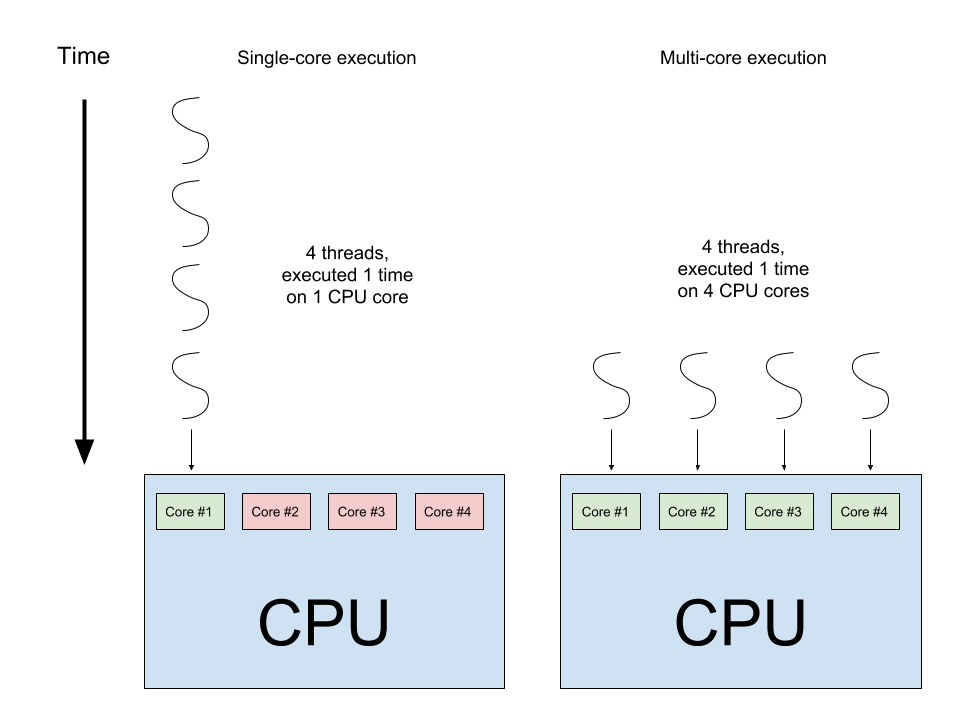
\includegraphics[width=0.9\linewidth]{Images/core_cores.png}
        \end{figure}
    \end{columns}

    \footnotenoindex{https://www.zhihu.com/question/25532384/answer/411179772}
    \footnotenoindex{https://blog.csdn.net/Victor2code/article/details/109005171}
    
\end{frame}

\begin{frame}{多进程与多线程}
    \begin{myoutline}
        \1 进程与线程的关系
            \2 线程在进程的管理下行进
                \3 单纯的车厢无法运行
            \2 一个进程可以包含多个线程
                \3 一辆火车可以有多个车厢
                \3 每个进程在执行过程中拥有独立的内存单元,而一个进程的多个线程在执行过程中共享内存
            \2 \textcolor{red}{进程要比线程消耗更多的计算机资源}
                \3 采用多列火车相比多个车厢更耗资源
            \2 进程间不会相互影响
                \3 一列火车不会影响到另外一列火车
            \2 一个线程挂掉将导致整个进程挂掉
                \3 一列火车上中间的一节车厢着火了,将影响到所有车厢
        \1 多核
            \2 多核CPU同时运行的线程可以属于单个进程或不同进程
            \2 进程使用的内存地址可以上锁
                \3 即一个线程使用某些共享内存时,其他线程必须等它结束,才能使用这一块内存。-"互斥锁"
        \1 \textcolor{red}{在大多数编程语言中},切换线程消耗的资源更少
            \2 而\textcolor{blue}{Python是个特例!}
    \end{myoutline}
\end{frame}


\begin{frame}{GIL锁}
    \begin{columns}
        \column{0.5\textwidth}
        \begin{myoutline}
            \1 GIL锁
                \2 Global Interpreter Lock, 全局解释器锁
                \2 GIL规定, 在一个进程中每次只能有一个线程在运行,也就是一个进程一把 GIL 锁
                    \3 这个GIL锁相当于是线程运行的资格证,某个线程想要运行,首先要获得GIL锁
                    \3 然后遇到IO或者超时的时候释放GIL锁, 给其余的线程去竞争
                    \3 竞争成功的线程获得GIL锁得到下一次运行的机会
            \1 GIL是个历史遗留问题
                \2 GIL的存在, 导致python的多线程其实是假的,所以才有人说python的多线程非常鸡肋
                \2 进程和进程之间会不会受影响?
                    \3 不会
        \end{myoutline}
        \column{0.5\textwidth}
        \begin{figure}
            \centering
            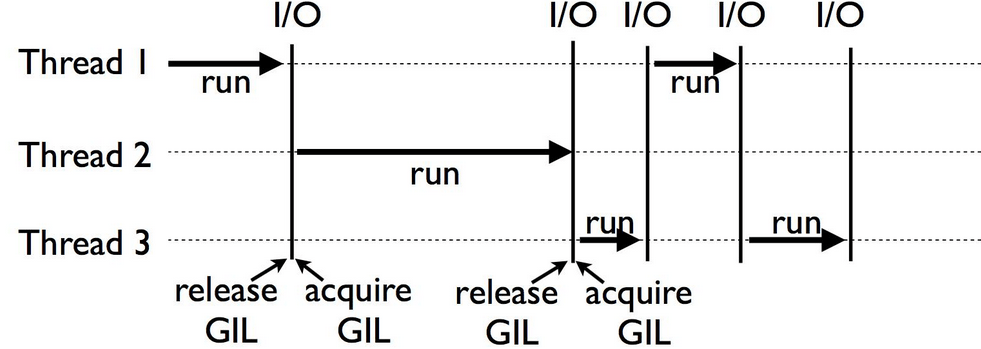
\includegraphics[width=0.9\linewidth]{Images/gil.png}
        \end{figure}
    \end{columns}
\end{frame}

\begin{frame}{由于 GIL 锁的存在}
    \begin{myoutline}
        \1 由于 GIL 锁的存在\dots
        \2 CPU密集型操作使用多进程比较合适, 例如海量运算, 测序 reads 比对到基因组, 计算给定区域的FPKM
        \2 IO密集型操作使用多线程比较合适, 例如爬虫, 超多文件处理
        \2 协程是线程的扩展, 进一步压榨 CPU 的算力(了解,可查阅 asyncio)
    \end{myoutline}
\end{frame}

\begin{frame}[standout]{练习多进程和多线程}
    \begin{myoutline}
        \1 多进程
        \1 多线程
        \1 进程的开销与线程的开销
        \1 进程池 Pool类
            \2 apply \& apply\_async
            \2 map \& map\_async
            \2 close, join, terminate
    \end{myoutline}
\end{frame}



% ————————————————
% 版权声明:本文为CSDN博主「T型人小付」的原创文章,遵循CC 4.0 BY-SA版权协议,转载请附上原文出处链接及本声明。
% 原文链接:https://blog.csdn.net/Victor2code/article/details/109005171